\lstset{ %
language=Python,                % the language of the code
basicstyle=\footnotesize,       % the size of the fonts that are used for the code
backgroundcolor=\color{white},  % choose the background color. You must add \usepackage{color}
showspaces=false,               % show spaces adding particular underscores
showstringspaces=false,         % underline spaces within strings
showtabs=false,                 % show tabs within strings adding particular underscores
frame=single,                   % adds a frame around the code
tabsize=2,                      % sets default tabsize to 2 spaces
captionpos=b,                   % sets the caption-position to bottom
breaklines=true,                % sets automatic line breaking
breakatwhitespace=false,        % sets if automatic breaks should only happen at whitespace
}


\section{Components}

What follows is a listing of application components.

\subsection{Stereo Calibrate}

Done by Jimi.

\subsection{Creating a model}



To create a model  of our 3d object we start out by determining the field we are going to use. For now, we do that using a A3 sized field with corners that are colored (in order) green, blue, red and black. \\
We use these corners to determine the orientation of our field. We do this by clicking on the corners in the image we get from the RGB camera, after we undistort the image. In stereo calibrate we found two intrinic matrices and two sets of distortion coefficients, a rotation matrix and a translation matrix. All these matrices can be used to undistort both images, so that an object in the depth image is in the same place as an object in the RGB image. We undistort the images using the InitUndistortRectifyMap function from OpenCV. \\
\\
Now the depth image and the RGB image are aligned and calibrated. In the create\_model.py module the user is asked to click on the pixels in the RGB image, where the corners of the A3 sized workingfield are (see Figure \ref{fig:clicking}).
\begin{figure}[H]
\centering
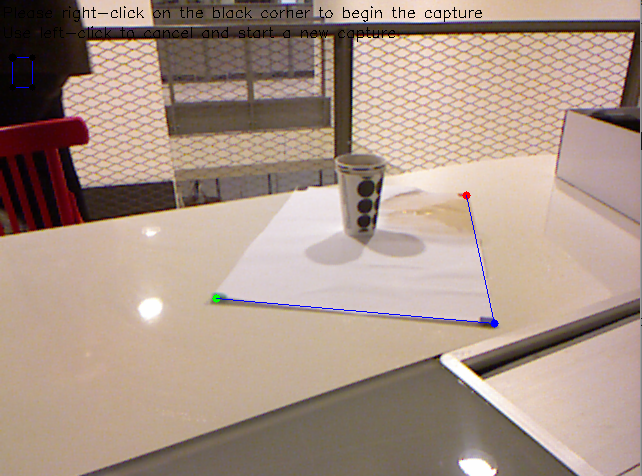
\includegraphics[scale=0.5]{images/clicking.png}
\caption{Clicking on the corners of the working field}
\label{fig:clicking}
\end{figure}
Since we have a depth image, we can make a working cube by taking the (x,y,z) value from the points (were the z value is derived from the depth image). The code displayed in \ref{code:cube} is applied to get all 8 points of a cube.\\
\begin{figure}[H]
\begin{lstlisting}
for i in xrange(4):
    cubic.append(np.array([points[i][0],points[i][1],sqrt(depth[points[i][1]][points[i][0]]]), dtype=float))
    if depth[points[i][1]][points[i][0]] > 2000:
        print "Point no. ", i, " is probably in a blind spot. Please start over."


for i in xrange(4):
    cubic = cubic + [np.cross((cubic[((i + 1) % 4)] - cubic[i]),(cubic[((i + 3) % 4)] - cubic[i]))]
    cubic[i + 4] = cubic[i + 4] / np.linalg.norm(cubic[i + 4])
    cubic[i + 4] = (cubic[i + 4] * height) + cubic[i]
\end{lstlisting}
\caption{The algorithm to create a 3 dimensional cube}
\label{code:cube}
\end{figure}
We don't really need the 4 points we calculated with the cross product for calculating the model. But the calculated cube is displayed in a wireframe on top of the rgb and depth image, so that the user can determine if the field is correct. At this point, the user can choose to start over or proceed with the points he/she clicked on. \\
\\
All the ingredients to start getting points for our 3d representation in points are now available:\\
\begin{itemize}
\item All matrices and coefficients for the rgb camera to calibrate (Found by stereo calibration)
\item All matrices and coefficients for the rgb camera to calibrate (Found by stereo calibration)
\item Four image points
\item A numpy array containing all RGB values at the moment when the first click was done
\item A numpy array containing all Depth values at the moment when the first click was done
\end{itemize}
For all points we found in the image, we need to determine the point in the object space. The object space is the cubic we found earlier, but we didn't determine the axis of the object space. Since we have clicked on all points of the A3 sized plane in a predetermined order, we can choose the axis of our cube. We chose the following: 
\begin{itemize}
\item The origin is in the point above the green corner
\item The x axis is the line that goes threw the origin and the point above the blue corner
\item The y axis is the line that goes threw the origin and the green corner
\item The z axis is the line that goes threw the origin and the point above the black corner
\end{itemize}
The result is visualized in \ref{fig:axis}. 
\begin{figure}[H]
\centering
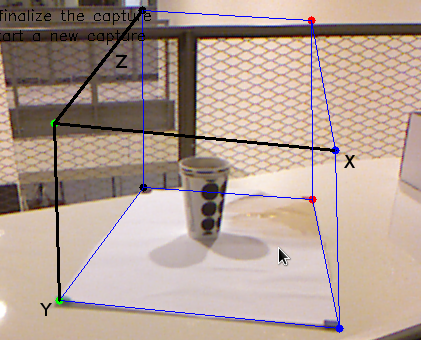
\includegraphics[scale=0.5]{images/axis.png}
\caption{Calculated cube, with axis}
\label{fig:axis}
\end{figure}




\subsection{Point Cloud Viewer}

The point cloud viewer was developed after examining various possible
bases, such as: PCL(see pointclouds.org, A very large production-class project for
anything to do with point clouds), PyGame and Visual. Visual is also know
as VPython.

For a very short period of time we tried using the mpl\_toolkit provided
by matplotlib, but as it has no support for OpenGL it isn't very suited
for rendering a large amount of points in 3D.

The PCL library was of course
very tempting, but very soon it became apparent this was way too much horse
power for our needs. What we needed was a simple interface that allowed viewing
of point clouds, rotating, moving and zooming them with mouse and keyboard
controls.

PyGame allows for very easy initialisation of OpenGL using SDL and can therefore
easily handle point clouds using most of today's graphics hardware. But it still
did not provide an easy way of controlling the camera. Rotation would require
using some sort of mathematical library implementing quaternion spherical rotation.

Enter VPython, a package attempting to implement a simple 3D programming
language on top of Python and allowing interactive terminal control of the
3D scene. VPython officially is composed of: Python (of course), IDLE the
interactive Python programming environment and the visual module. When we
discoverd the visual module used OpenGL, offers mouse orientation
controls by default, and to top it off uses NumPy for all its data manipulation
our course of action became very clear. Since the Kinect library provides its
data in NumPy arrays, after simple manipulation the point clouds can be fed into
visual with the simple command "points".

Currently the point cloud viewer does not support realtime capture, but capture
is done quickly and easily using the 'c' key.


The low-level interface includes the option for depth smoothing.

\subsection{Combining it all}
